\section{Resultados preliminares}
\subsection{Objetivos experimentos}

%todo: completar con la 
En esta sección de forma preliminar, se busca comparar la calidad de las soluciones obtenidas por el algoritmo propuesto comparados dos algoritmos: \textit{Best path dijkstra} y \textit{Static shortest path}  de la literatura en \cite{Yuan20091081}.
Además se construye un nuevo set de instancias basada en el trabajo \cite{forcael2014ant}.


\subsection{Instancias de pruebas}


\subsubsection{Yuan}
En \cite{Yuan20091081} se presenta una red de 20 nodos divididos en 3 áreas como se muestra en la figura \ref{area3}. En cada área los parámetros son generados de forma aleatoria. Estos se observan en el cuadro \ref{table:intervalo}. Para el desastre 0, una situación sin ningún desastre y el desastre 4 es una situación más compleja. Para las instancias propuestas por \cite{Yuan20091081} se considera que el nodo 20 es un nodo seguro.

\begin{figure}[H]
\centering
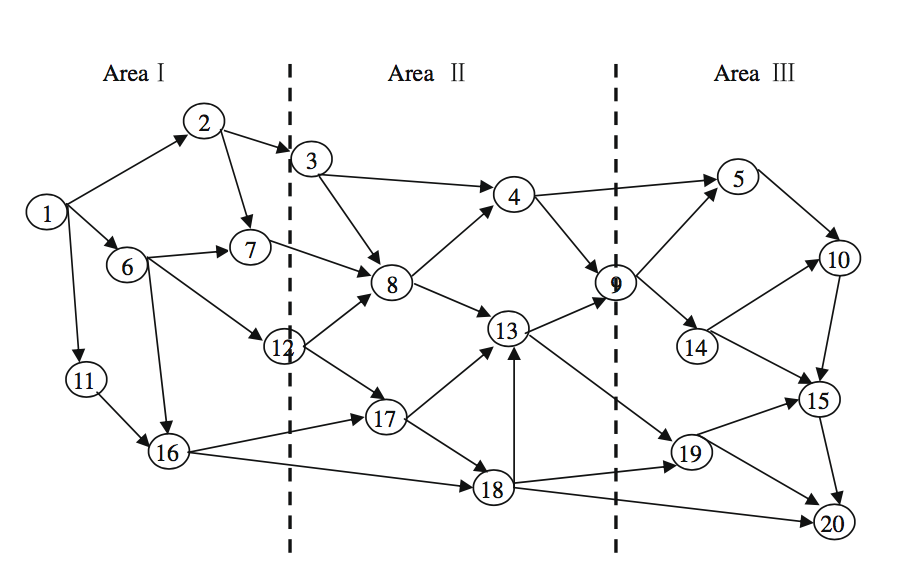
\includegraphics[scale=0.5]{images/areas.jpg}
\caption{División de una red de emergencia}\label{area3}

\end{figure}

En los cuadros \ref{grade1}, \ref{grade2}, \ref{grade3} y \ref{grade4} se muestran los valores correspondientes al nodo $i$ y nodo $j$. $l_{i,j}$ $s_{i,j}^0$, $\alpha_{ij}$ y $\beta_{ij}$ según los distintos grados de desastre.



\begin{table}[H]
\centering
\begin{tabular}{|l|l|l|l|}
\hline
Tipo & Área I & Área II & Área III \\ \hline
Desastre 0 & $\alpha=1$,$\beta=0$ & $\alpha=1$,$\beta=0$ & $\alpha=1$,$\beta=0$ \\ \hline
Desastre 1 & $\alpha \in (0.9,1.0)$ $\beta \in (0.00,0.05)$ & $\alpha=1$,$\beta=0$ & $\alpha=1$,$\beta=0$ \\ \hline
Desastre 2 & $\alpha \in (0.8,0.9)$ $\beta \in (0.05,0.10)$ & $\alpha \in (0.9,1.0)$ $\beta \in (0.00,0.05)$ & $\alpha=1$,$\beta=0$ \\ \hline
Desastre 3 & $\alpha \in (0.7,0.8)$ $\beta \in (0.10,0.15)$ & $\alpha \in (0.8,0.9)$ $\beta \in (0.05,0.10)$ & $\alpha \in (0.9,1.0)$ $\beta \in (0.00,0.05)$ \\ \hline
Desastre 4 & $\alpha \in (0.6,0.7)$ $\beta \in (0.15,0.20)$ & $\alpha \in (0.7,0.8)$ $\beta \in (0.10,0.15)$ & $\alpha \in (0.8,0.9)$ $\beta \in (0.05,0.10)$ \\ \hline
\end{tabular}
\caption{Intervalos de los parametros por área}\label{table:intervalo}
\end{table}

\subsubsection{Penco}

En \cite{forcael2014ant} se presenta una red de 67 nodos representando la ciudad de Penco de Chile, cada nodo representa una esquina de la ciudad considerando el nodo 67 como una zona segura. En el cuadro \ref{tab:penco}